\section{Introduction}
\begin{frame}{Motivation}
    \begin{columns}[T]
    \column{1.0\textwidth}
    \raggeditems
    \begin{itemize}
        % \item Centralized platforms run on \emph{surveillance capitalism}: monetization of user data~\cite{Zuboff2023}
        % \item Internet shutdowns are a routine tool of \emph{networked autocracy}: governmental control of information, finance, media institutions~\cite{Lopez2026, Sarvestany2026, Bitchat-nepal, Bitchat-iran-uganda}
        % \item \emph{War and disasters} disrupt the physical network~\cite{gaza-brief,Aceto2026}
        \item Social networks that depend on any party but its members can be shut down.        
        \item Shutdowns, disasters, surveillance and control happen~\cite{Aceto2026,Lopez2026,Sarvestany2026,Zuboff2023}
        \item Use offline-first local communication, augmented with Internet instead of dependent on it
    \end{itemize}
    \end{columns}
    \vspace{2ex}
    \begin{columns}[T]
    \column{0.32\textwidth}
    \centering
    
\includegraphics[height=2.1cm]{pics/surveillance-capitalism.jpg}\\{\tiny Harvard Gazette}
    \column{0.32\textwidth}
    \centering
    
\includegraphics[height=2.1cm]{pics/networked-autocracy.jpg}\\{\tiny ECFR}
    \column{0.32\textwidth}
    \centering
    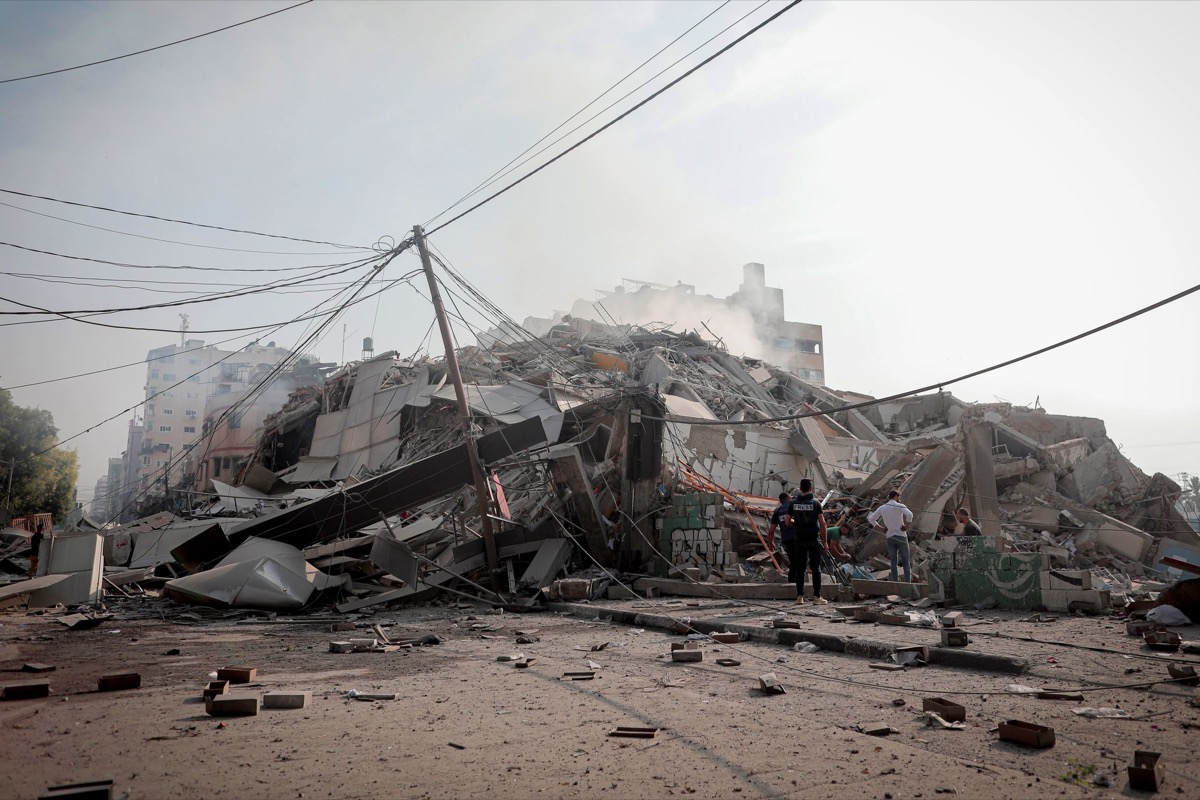
\includegraphics[height=2.1cm]{pics/gaza-outage.jpg}\\{\tiny Getty Images / WIRED}
    \end{columns}
\end{frame}
\begin{frame}{Problems}
    \noindent{\small$\Pi$ is every agent that could take part. A set $E\subseteq\Pi$ is \textbf{essential} if it is the minimal one whose removal leaves every remaining agent unable to interact with anyone; the smallest such $|E|$ sorts every platform into four classes~\cite[Def.~2.9,~2.10]{Shapiro2026Platforms}.}
    \par\vspace{0.5ex}
    \centering
    \small
    \setlength{\tabcolsep}{3pt}
    \begin{tabular}{@{}lY{1.7cm}Y{3.8cm}Y{2.7cm}@{}}
        \toprule
        Class & Example & Essential agents & cardinality \\
        \midrule
        Centralized & Facebook & the operator's own server~\cite{Lopez2026} & $|E|=1$ \\
        \midrule
        \multicolumn{4}{@{}l}{\emph{Distributed}~\cite{Jeong2025}} \\ \addlinespace[1.5ex]
        \quad Federated & Mastodon & \multirow{2}{=}{\raggedright instances, and bootstrap nodes: infinite, but not universal~\cite{Aravindh2019, Li2019}} &$|E|=\infty$, $|\Pi\setminus E|\ge 2$\\
        \quad Blockchain & Steemit & &$|E|=\infty$\\ \addlinespace[3ex]
        \quad Peer-to-peer & Briar, BitChat & Tor or Nostr relays~\cite{briar, bitchat} & $1<|E|<\infty$ \\
        \midrule
        \textbf{Grassroots} & \textbf{SSB, GNL} & \textbf{everyone}~\cite{Tarr2019, Shapiro2023} & $\Pi$\\
        \bottomrule
    \end{tabular}
    \par\vspace{0.5ex}
    \takeaway{A GSN has $|E|=\Pi\setminus\{p\}$: we chose to model our system after GSNs as universal set, having no central infrastructure}
\end{frame}

\begin{frame}{Background: OppNets}
    \begin{columns}[T]
    \column{0.56\textwidth}
    \raggeditems
    \begin{itemize}
        \item MANETs need a connected end-to-end path, which a crisis zone never offers~\cite{RFC2501, Conti2014}
        \item Opportunistic networks \emph{store, carry, forward} until a contact arises~\cite{Pelusi2006, RFC4838}
        \item Structured overlays give lower latency and a global state, but lean on designated nodes and degrade under churn~\cite{kademlia, chord, Lua2005}
        \item Unstructured overlays tolerate churn at the price of gossip overhead~\cite{Lua2005, guzman25}
        % \item Epidemic flooding delivers the most and congests first~\cite{Vahdat2000}
    \end{itemize}
    \column{0.42\textwidth}
    \centering
    \vspace{3mm}
    \begin{tikzpicture}[x=0.8mm,y=0.8mm, font=\scriptsize,
        dev/.style={circle, draw, thick, fill=white, minimum size=4.5mm, inner sep=0pt},
        lnk/.style={thick, TUMBlue}]
        \draw[dashed, black!50] (6,14) ellipse (11 and 12);
        \draw[dashed, black!50] (44,14) ellipse (11 and 12);
        \node[dev] (a1) at (1,14) {S};
        \node[dev] (a2) at (9,21) {};
        \node[dev] (a3) at (9,7) {};
        \draw[lnk] (a1)--(a2) (a1)--(a3) (a2)--(a3);
        \node[dev] (b1) at (49,14) {D};
        \node[dev] (b2) at (41,21) {};
        \node[dev] (b3) at (41,7) {};
        \draw[lnk] (b1)--(b2) (b1)--(b3) (b2)--(b3);
        \node[dev, fill=TUMOrange!30] (c) at (18,14) {C};
        \node[dev, fill=TUMOrange!30, dashed] (c2) at (32,14) {C};
        \draw[lnk, dashed] (a3)--(c);
        \draw[->, thick, TUMOrange] (c) -- (c2) node[midway, above] {carry};
        \draw[lnk, dashed] (c2)--(b3);
        \node[font=\scriptsize, TUMOrange, below=0.6mm of c] {store};
        \node[font=\scriptsize, TUMOrange, below=0.6mm of c2] {forward};
        \node[font=\scriptsize, black!60, align=center] at (25,-3) {no end-to-end path ever exists between S and D};
    \end{tikzpicture}
    \captionof{figure}{Store, carry, forward}
    \end{columns}
    \takeaway{Model GSN as OppNet with Store-carry-forward best effort delivery!}
\end{frame}

\begin{frame}{Solution Approach}
    \begin{moepdef}{blue}{filled}{Research question}
        What must be added to a BLE mesh, without introducing third party infrastructure, for a grassroots social network to deliver at scale?
    \end{moepdef}\par
    \vspace{1.5ex}
    \textbf{Contributions}
    \begin{itemize}
            % \item \textbf{Build} the networking layer: one application-layer overlay over a physical-layer local-area underlay and a transport-layer wide-area underlay
            \item \textbf{Measure} the grassroots networking layer on a testbed of commodity smartphones: what a link costs, how delivery degrades under contention, how often links flap
            \item \textbf{Simulate} at scale, calibrated on those measurements, to compare control-plane and forwarding strategies
            \item \textbf{Results} we found that contention collapses delivery even at close range, link outages are common on old hardware and heavy-tailed, and BLE-only saturates at 80\% delivery, with the Internet addition bridging to 100\%
    \end{itemize}
\end{frame}

\begin{frame}{Related Works}
    \begin{center}
    \small
    \setlength{\tabcolsep}{5pt}
    \begin{tabular}{@{}Y{2.2cm}Y{3.6cm}Y{2.6cm}Y{2.5cm}@{}}
        \toprule
        System & Local-area underlay & Wide-area underlay & Third-party dependency \\
        \midrule
        SSB~\cite{Tarr2019} & WLAN, Bluetooth Classic\textsuperscript{*} & pub servers over TCP&pub servers\\
        Briar~\cite{briar} & WLAN, Bluetooth Classic & Tor & Tor~\cite{Aceto2026} \\
        BitChat~\cite{bitchat} & BLE mesh & Nostr relays & the relays~\cite{Wei2025} \\
        Amigo~\cite{Inyangson2025} & Wi-Fi Direct & none & GPS \\
        % \midrule
        % \textbf{GNL} & BLE mesh, controlled flooding with custody & UDX streams between friends, NAT hole punching & none: friends act as rendezvous agents \\
        \bottomrule
    \end{tabular}
    \end{center}
    \begin{itemize}
        \item The component structure inherits from BitChat; Nostr relays replaced by edge rendezvous points (friends) for hole-punching
        % s\item Information travels along the edges of the social graph~\cite{Shapiro2023}
    \end{itemize}
\end{frame}
